\documentclass[../main.tex]{subfiles}

\begin{document}

\chapter{Intercellular communication as a series of narrow escape problems}
\label{cha:narrowescape}



\begin{figure}[!ht]
  \centering
     \subfloat[First sub-figure\label{subfig-1:nrescp}]{%
       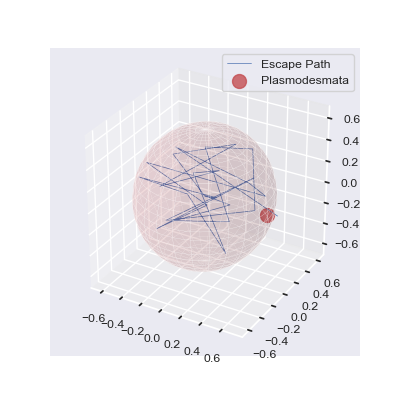
\includegraphics[width=0.3\columnwidth]{./figures/escape_example.png}
     }
     \hfill
     \subfloat[First sub-figure\label{subfig-2:nrescp}]{%
       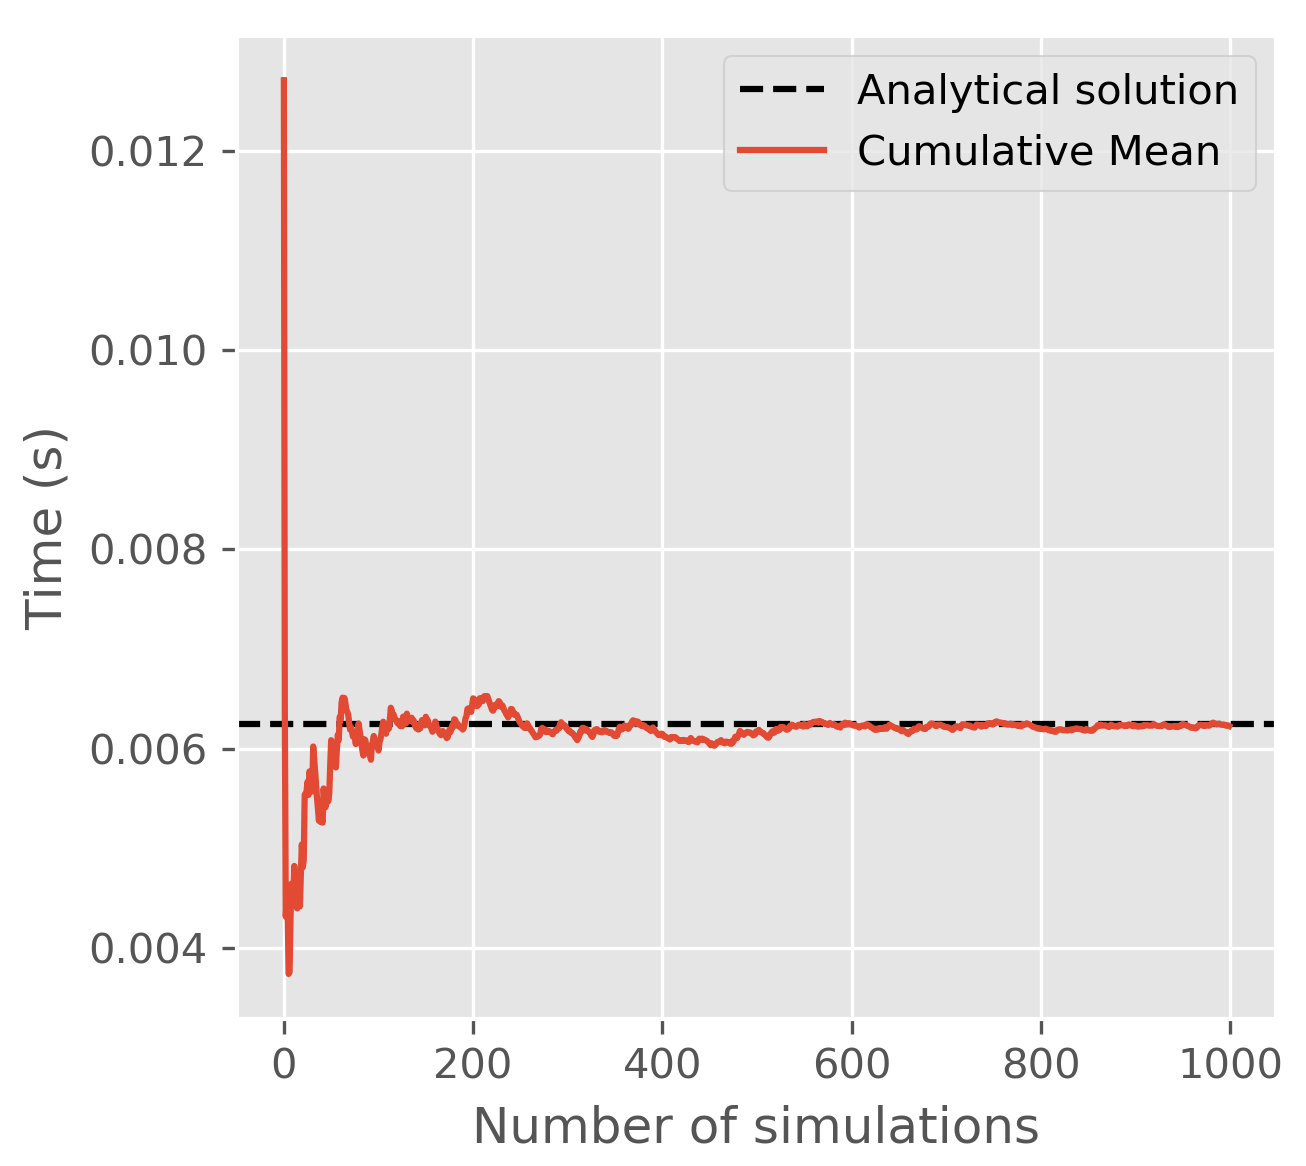
\includegraphics[width=0.3\columnwidth]{./figures/cummean.png}
     }
     \hfill
     \subfloat[First sub-figure\label{subfig-3:nrescp}]{%
       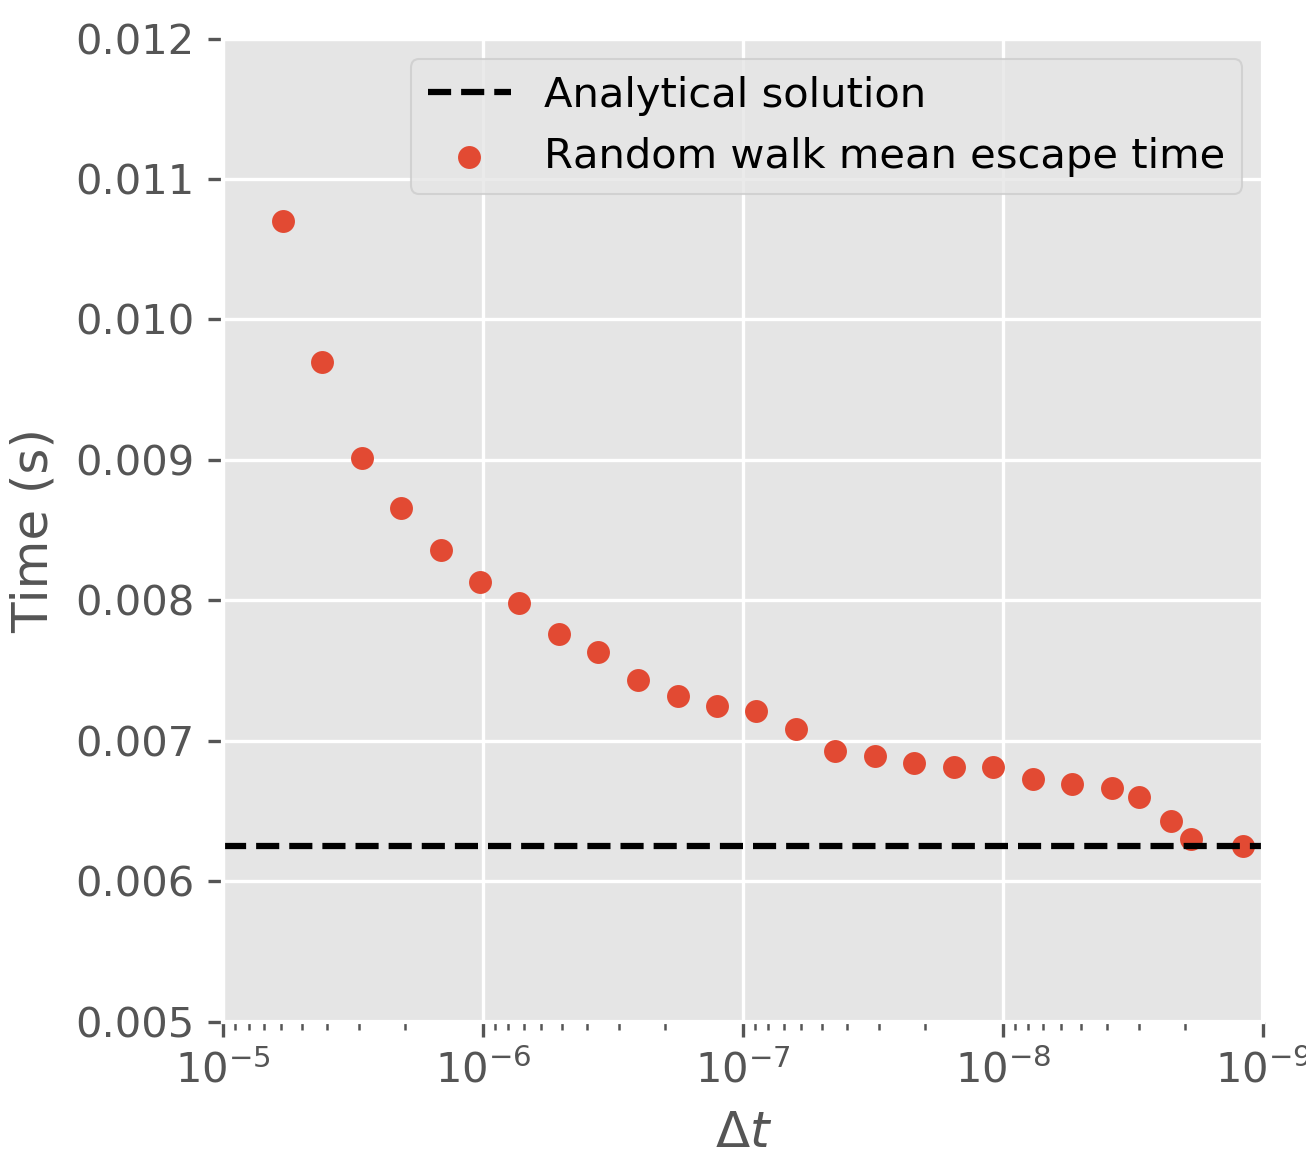
\includegraphics[width=0.3\columnwidth]{./figures/deltat.png}
     }
     \caption{Narrow escape confirmations}
     \label{fig:nrescp}
   \end{figure}



  
\begin{figure}[!ht]
  \centering
     \subfloat[First sub-figure\label{subfig-1:nrescp2}]{%
       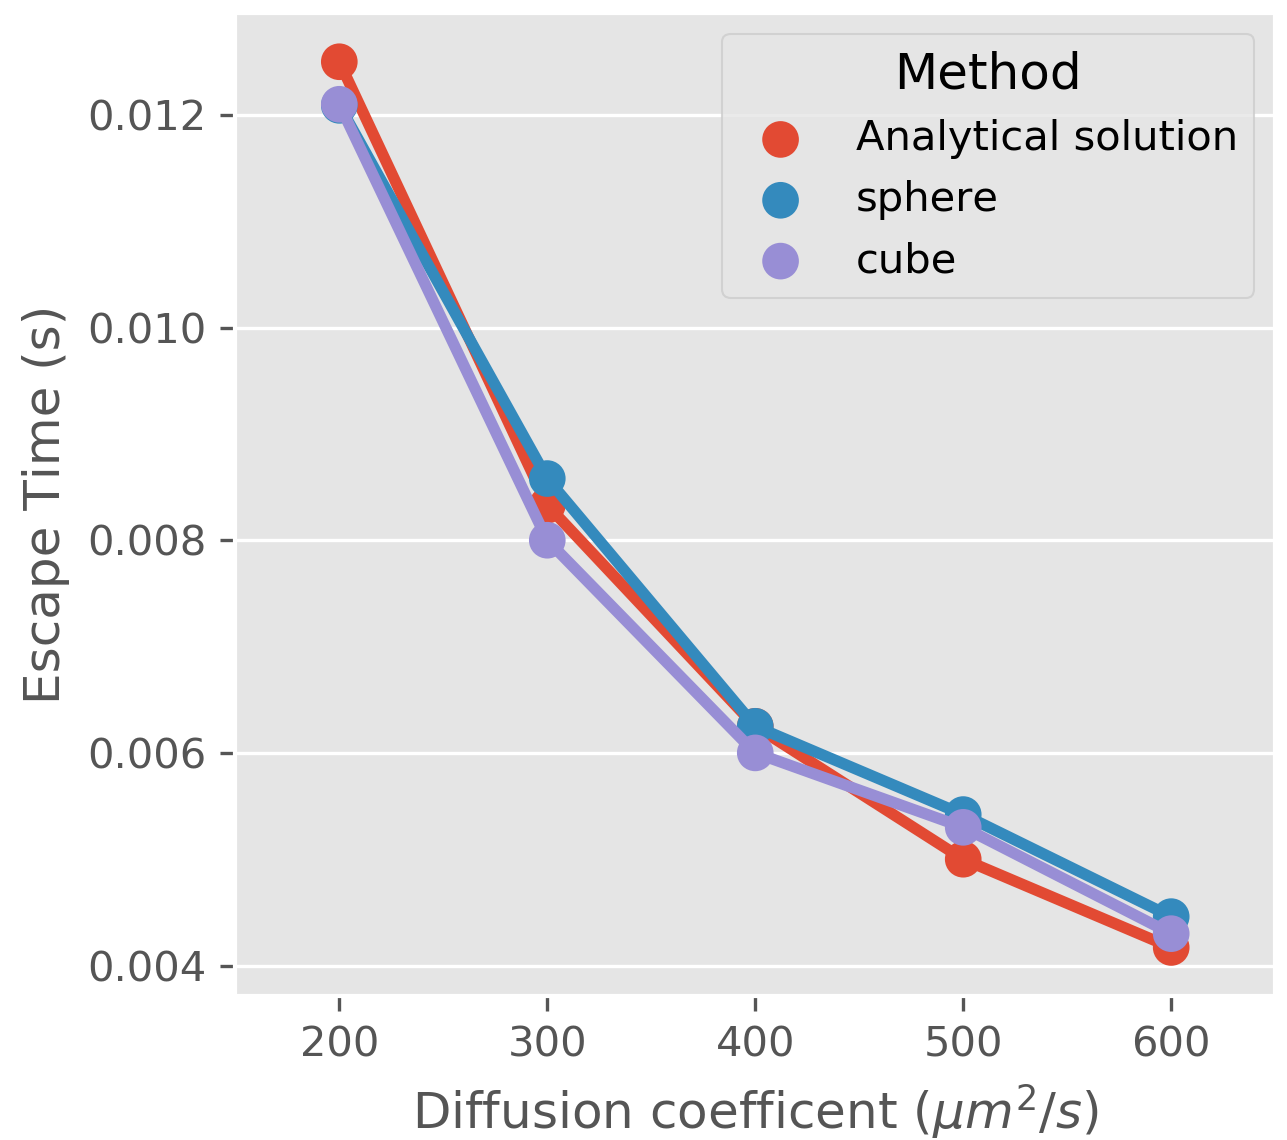
\includegraphics[width=0.3\columnwidth]{./figures/escpD.png}
     }
     \subfloat[First sub-figure\label{subfig-2:nrescp2}]{%
       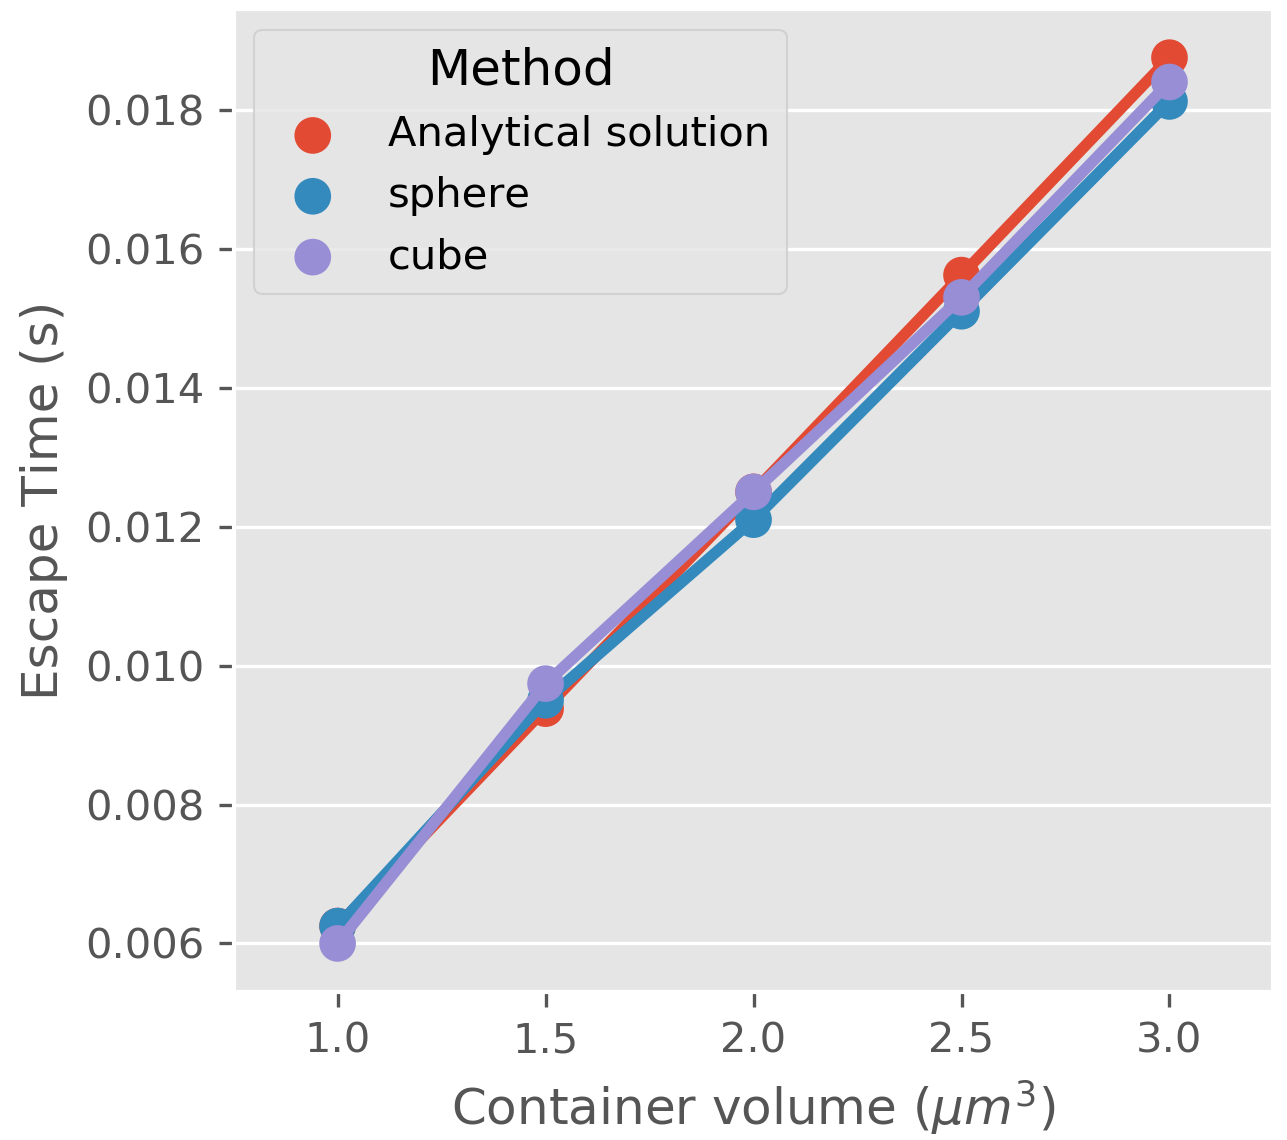
\includegraphics[width=0.3\columnwidth]{./figures/escpV.png}
     }
     \caption{Narrow escape parameters}
     \label{fig:nrescp2}
   \end{figure}



   

\end{document}


%%% Local Variables:
%%% mode: latex
%%% TeX-master: "../main"
%%% End:
